\documentclass[10pt]{beamer}
\usetheme{jambro}

\title[]{Macroeconomia I - Mercados Financeiros}
\author[]{Paulo Victor da Fonseca}
\date{}

\hypersetup{
    colorlinks = true,
    urlcolor = teal,
    linkcolor = teal    
}
\usepackage[portuguese]{babel}
\usepackage{subfig}
\usepackage{emoji}
\usepackage{hyperref}

\begin{document}

\begin{frame}[plain]
    \titlepage{
        \begin{center}
            \begin{minipage}{0.8\textwidth}
                \centering
            \end{minipage}
        \end{center}}
\end{frame}

\begin{frame}{Sumário}
    \tableofcontents
\end{frame}

\section{Introdução}
\begin{frame}{Introdução}
    \begin{itemize}
        \item Aulas anteriores: determinação do equilíbrio no mercado de bens e serviços
        \bigskip
        \item Objetivo, agora, estudar mercados financeiros e como operações do Banco Central (BC) afetam as taxas de juros
        \bigskip
        \item Os mercados financeiros envolvem uma rede intrincada de instituições (bancos, fundos do mercado monetário, fundos mútuos, fundos de investimento e fundos \emph{hedge})
        \bigskip
        \item As transações envolvem títulos, ações e outros créditos financeiros como \emph{swaps} e opções
        \bigskip
        \item Além disso, existe um conjunto enorme de taxas de juros: taxas de juros de muitos tipos diferentes de títulos do governo, diversos títulos corporativos, de títulos de curto prazo, de títulos de longo prazo, etc
    \end{itemize}
\end{frame}

\begin{frame}{Introdução}
    \begin{itemize}
        \item Os mercados financeiros desempenham um papel fundamental na economia, determinam os custos dos fundos para empresas, famílias e governo e, consequentemente, afetam suas decisões de gastos
        \bigskip
        \item Como nosso objetivo é estudar o papel do BC em afetar as taxas de juros, consideraremos um modelo super simplificado de uma economia com apenas dois ativos: moeda (que não paga juros) e títulos (que pagam)
        \bigskip
        \item Isso nos permitirá entender como a taxa de juros dos títulos é determinada e o papel do BC nesta determinação
    \end{itemize}
\end{frame}

\section{Demanda por moeda}
\subsection{Moeda, renda e riqueza}
\begin{frame}{Moeda, renda e riqueza}
    \begin{itemize}
        \item \textcolor{blue}{Moeda:} é o que se pode usar para pagar transações e pode ser papel-moeda ou depósitos à vista em bancos
        \bigskip
        \item \textcolor{blue}{Renda:} é o que se ganha com o trabalho mais o que se recebe em juros e dividendos. A renda é uma variável de \textbf{fluxo}, ou seja, algo expresso em unidades de tempo (renda mensal, renda anual, etc.)
        \bigskip
        \item \textcolor{blue}{Riqueza financeira:} ou simplesmente riqueza, é o valor de todos os ativos financeiros menos todos os passivos financeiros. A riqueza é uma variável de \textbf{estoque}, ou seja, é o valor da riqueza em dado instante do tempo
        \bigskip
        \item Em dado instante do tempo não se pode alterar o montante total da riqueza financeira. Só se pode fazer isso ao longo do tempo, à medida que se poupa e despoupa, ou à medida que os valores dos ativos e passivos variam
    \end{itemize}
\end{frame}

\begin{frame}{Moeda, renda e riqueza}
\begin{itemize}
    \item É possível, no entanto, mudarmos a composição da riqueza em um dado instante do tempo. E.g., podemos pagar parte da hipoteca emitindo um cheque da conta-corrente. Isto leva a uma diminuição dos passivos (hipoteca menor) e a uma diminuição equivalente dos ativos (um saldo menor em conta-corrente). Enquanto mantem a riqueza inalterada
    \bigskip
    \item Os ativos financeiros que podem ser usados diretamente para comprar bens são chamados de \emph{moeda} e incluem o papel-moeda e os depósitos à vista, ou seja, depósitos contra os quais se pode emitir cheques. A moeda também é uma variável de estoque
\end{itemize}
\end{frame}

\subsection{Demanda por moeda}
\begin{frame}{Demanda por moeda}
    \begin{itemize}
        \item Suponha que um indivíduo, por ter poupado regularmente parte de sua renda no passado, possua uma riqueza financeira atual de \$50.000
        \bigskip
        \item Este indivíduo pode continuar poupando no futuro e, com isso, aumentar sua riqueza. No entanto, seu valor atual já está determinado
        \bigskip
        \item Por hipótese, vamos supor que este indivíduo pode decidir como alocar sua riqueza financeira somente entre dois tipos de ativos - moeda e títulos
    \end{itemize}
\end{frame}

\begin{frame}{Demanda por moeda}
    \begin{itemize}
        \item A \textcolor{blue}{moeda}, que pode ser usada para transações, não paga juros. Existem dois tipos de moeda: \textbf{papel-moeda} - moedas e notas em espécie - e \textbf{depósitos à vista} - os depósitos bancários sobre os quais é possível emitir cheques ou utilizar o cartão de débito
        \bigskip
        \item Os \textcolor{blue}{títulos}, por sua vez, pagam uma taxa de juros positiva, $i$, mas não podem ser usados em transações. Cabe ressaltar que, no mundo real, há muitos tipos de títulos, cada qual associado a uma taxa de juros específica. Por enquanto, vamos ignorar este aspecto da realidade e considerar que haja apenas um tipo de título que pague uma taxa de juros $i$
    \end{itemize}
\end{frame}

\begin{frame}{Demanda por moeda}
    \begin{itemize}
        \item Vamos supor que a compra e venda de títulos implique algum custo - e.g., taxa de corretagem
        \bigskip
        \item Quanto de sua riqueza financeira de \$50.000 este indivíduo deveria reter em moeda e quanto em títulos?
        \bigskip
        \begin{enumerate}
            \item Manter toda a riqueza sob forma de moeda é conveniente. Mas isto implica em não receber nenhuma renda em juros
            \bigskip
            \item Manter toda a riqueza sob forma de títulos é bastante inconveniente, mesmo que este indivíduo receba juros sobre o montante total. Isto porque deverá contatar seu corretor frequentemente para qualquer transação que precisar fazer no dia a dia
        \end{enumerate}
    \end{itemize}
\end{frame}

\begin{frame}{Demanda por moeda}
    \begin{itemize}
        \item Portanto, este indivíduo deveria alocar sua riqueza tanto em moeda quanto em títulos
        \bigskip
        \item Para respondermos em qual proporção, devemos considerar as seguintes duas variáveis:
        \bigskip
        \begin{enumerate}
            \item \textcolor{blue}{Nível de transações:} o indivíduo desejará ter moeda suficiente à disposição para evitar a venda frequente de títulos em troca de moeda
            \bigskip
            \item \textcolor{blue}{Taxa de juros dos títulos:} o único motivo para reter parte da riqueza em títulos é que eles pagam juros. Quanto mais alta a taxa de juros, mais disposto este indivíduo estará a enfrentar o trabalho e custos associados à compra e venda de títulos
        \end{enumerate}
    \end{itemize}
\end{frame}

\subsection{Derivação da demanda por moeda}
\begin{frame}{Derivação da demanda por moeda}
\begin{itemize}
    \item Seja o montante de moeda que as pessoas desejam reter - sua \textcolor{blue}{demanda por moeda} - dado por $M^d$. A demanda por moeda na economia é a soma de todas as demandas por moeda individuais
    \bigskip
    \item Portanto, ela depende do nível total de transações na economia e da taxa de juros
    \bigskip
    \item A mensuração do nível total de transações na economia é difícil de ser obtida. Mas podemos usar a renda agregada nominal como uma \emph{proxy}
    \bigskip
    \item Portanto, a relação entre a demanda por moeda, renda nominal e taxa de juros pode ser descrita pela seguinte equação:
    \begin{equation}
        M^d = \$Y L(i), \qquad L'(i) < 0.
        \label{eq1}
    \end{equation}
    em que $\$ Y$ representa a renda nominal
\end{itemize}
\end{frame}

\begin{frame}{Derivação da demanda por moeda}
    \begin{itemize}
        \item A demanda por moeda, $M^d$, é igual à renda nominal, $\$Y$, multiplicada por uma função da taxa de juros, $i$, representada por $L(i)$:
        \bigskip
        \begin{enumerate}
            \item A demanda por moeda aumenta em proporção à renda nominal. Se a renda nominal dobra, a demanda por moeda também dobra
            \bigskip
            \item A demanda por moeda depende negativamente da taxa de juros, ou seja, um aumento na taxa de juros diminui a demanda por moeda
        \end{enumerate}
    \end{itemize}
\end{frame}

\begin{frame}{Derivação da demanda por moeda}
    \begin{figure}
        \centering
        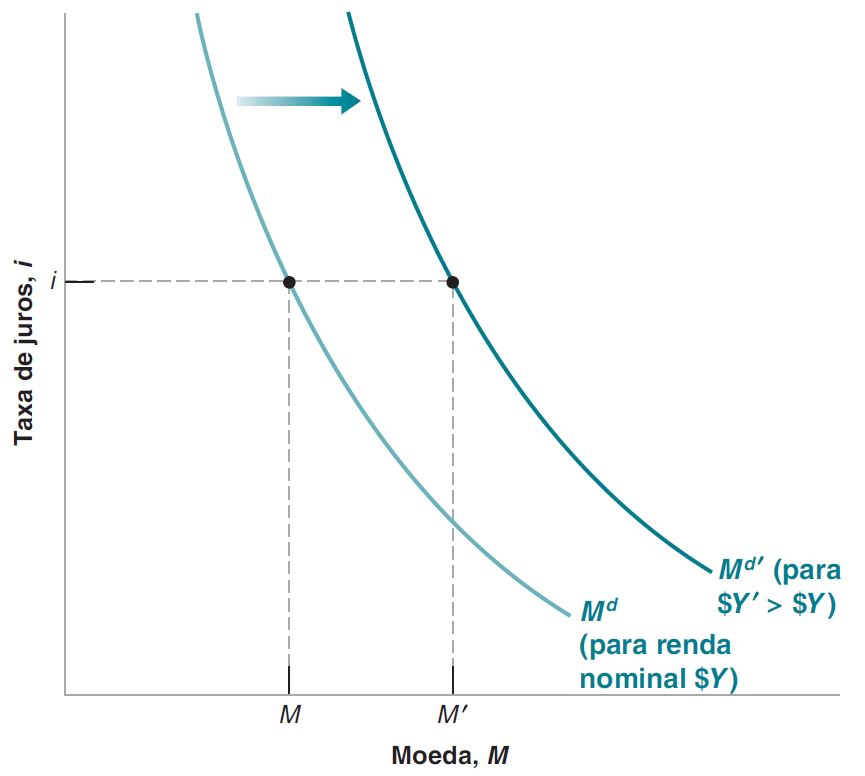
\includegraphics[width=0.5\textwidth]{./figures/aula072_fig1.JPG}
        \caption{Demanda por moeda. Fonte: Blanchard (2017).}
        \label{fig1}
    \end{figure}
\end{frame}

\section{Determinação da taxa de juros (I)}
\subsection{Determinação da taxa de juros}
\begin{frame}{Demanda por moeda, oferta de moeda e taxa de juros de equilíbrio}
    \begin{itemize}
        \item Moeda: depósitos à vista (ofertados pelos bancos) e papel-moeda (ofertada pelo BC)
        \bigskip
        \item Por simplicidade, consideraremos, inicialmente, que a oferta de moeda é dada apenas pelo papel-moeda
        \bigskip
        \item Vamos supor que o Banco Central decida ofertar um montante de moeda igual a $M$, de modo que:
        \[
        M^s = M.
        \]
    \end{itemize}
\end{frame}

\begin{frame}{Demanda por moeda, oferta de moeda e taxa de juros de equilíbrio}
\begin{itemize}
    \item Equilíbrio nos mercados financeiros:
    \begin{equation}
        M = \$Y L(i).
        \label{eq3}
    \end{equation}
    \bigskip
    \item A taxa de juros $i$ deve ser tal que, dada a renda nominal, as pessoas estejam dispostas a ter um montante de moeda igual à oferta de moeda existente $M$
\end{itemize}
\end{frame}

\begin{frame}{Demanda por moeda, oferta de moeda e taxa de juros de equilíbrio}
\begin{figure}
    \centering
    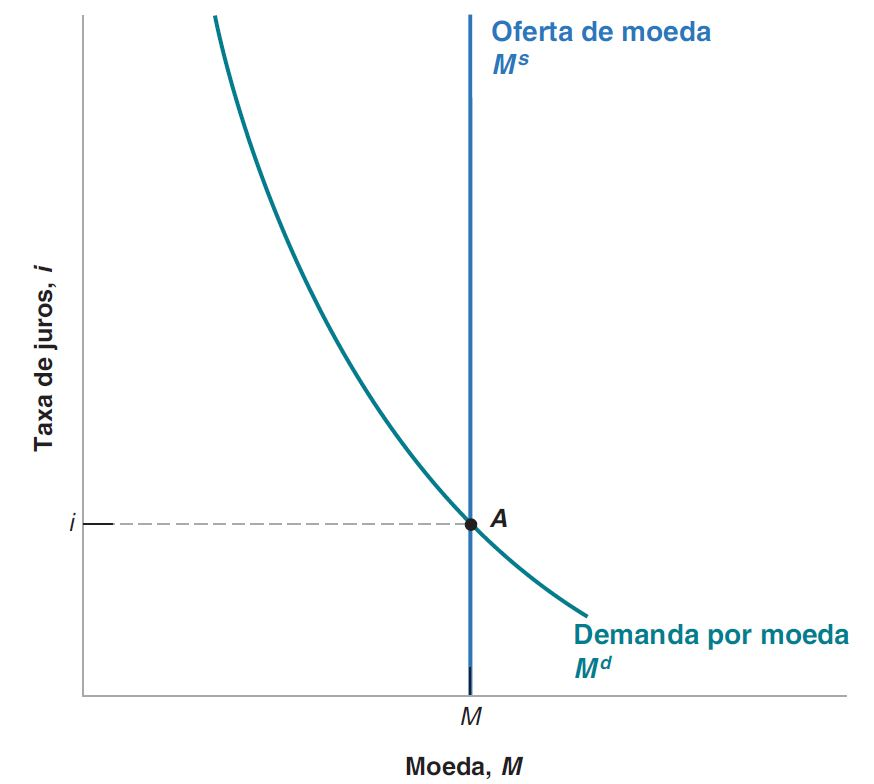
\includegraphics[width=0.5\textwidth]{./figures/aula072_fig2.JPG}
    \caption{Determinação da taxa de juros. Fonte: Blanchard (2017).}
    \label{fig2}
\end{figure}
\end{frame}

\begin{frame}{Efeitos de um aumento na renda nominal sobre a taxa de juros}
    \begin{figure}
        \centering
        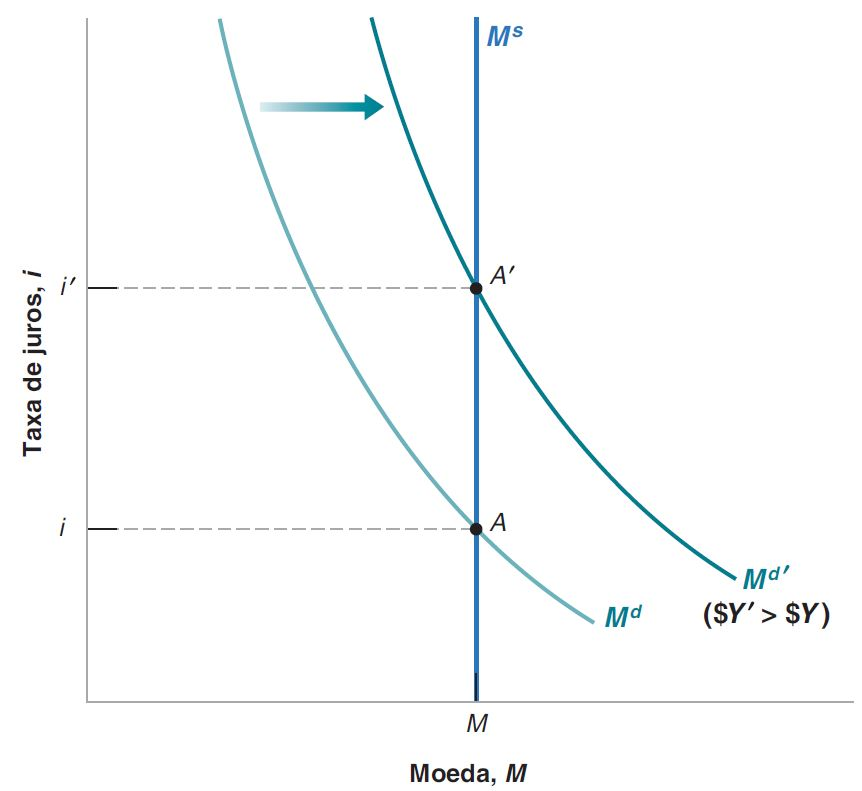
\includegraphics[width=0.5\textwidth]{./figures/aula072_fig3.JPG}
        \caption{Efeitos de um aumento na renda nominal sobre a taxa de juros. Fonte: Blanchard (2017).}
        \label{fig3}
    \end{figure}
\end{frame}

\begin{frame}{Efeitos de um aumento na renda nominal sobre a taxa de juros}
\begin{itemize}
    \item Aumento da renda nominal de $\$Y$ para $\$ Y^{'}$ aumenta o nível de transações, que aumenta a demanda por moeda a qualquer taxa de juros
    \bigskip
    \item A curva de demanda por moeda se desloca para a direita, de $M^d$ para $M^{d'}$
    \bigskip
    \item O equilíbrio se move para cima, de $A$ para $A^{'}$, e a taxa de juros de equilíbrio aumenta de $i$ para $i^{'}$
    \bigskip
    \item Para uma dada oferta de moeda exógena, um aumento da renda nominal leva a um aumento da taxa de juros de equilíbrio
    \bigskip
    \item À taxa de juros inicial, a demanda por moeda excede a oferta. Logo, um aumento da taxa de juros é necessário para diminuir o montante de moeda que as pessoas desejam reter e para restabelecer o equilíbrio
\end{itemize}
\end{frame}

\begin{frame}{Efeitos de um aumento da oferta de moeda sobre a taxa de juros}
    \begin{figure}
        \centering
        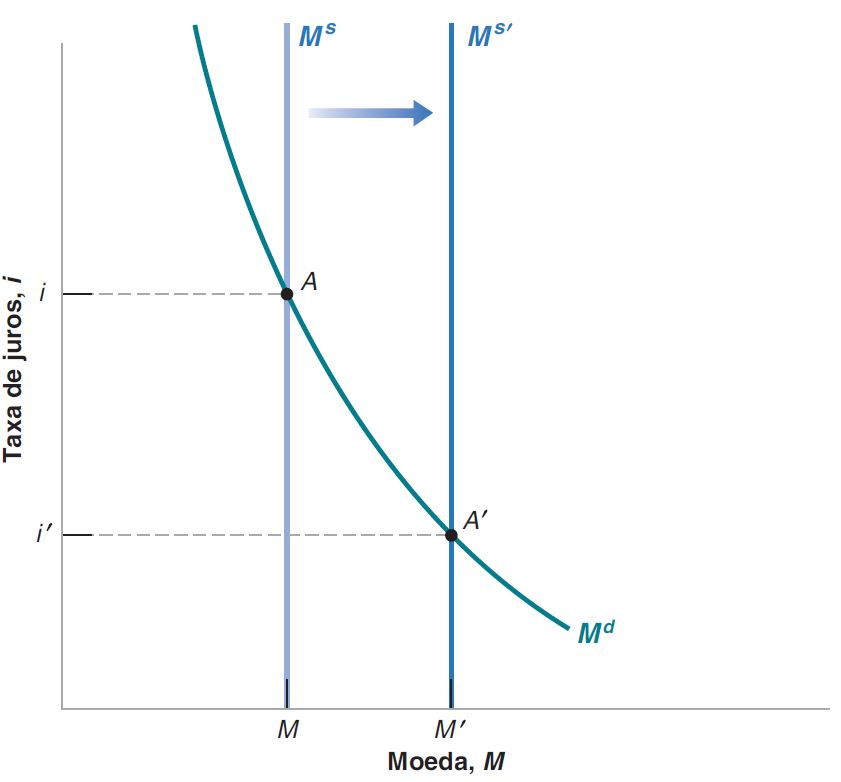
\includegraphics[width=0.5\textwidth]{./figures/aula072_fig4.JPG}
        \caption{Efeitos de um aumento da oferta de moeda sobre a taxa de juros. Fonte: Blanchard (2017).}
        \label{fig4}
    \end{figure}
\end{frame}

\begin{frame}{Efeitos de um aumento da oferta de moeda sobre a taxa de juros}
\begin{itemize}
    \item Um aumento da oferta de moeda leva a um deslocamento da curva de oferta de moeda para a direita, de $M^s$ para $M^{s'}$
    \bigskip
    \item O equilíbrio se move para baixo, de $A$ para $A^{'}$, e a taxa de juros de equilíbrio diminui de $i$ para $i^{'}$
    \bigskip
    \item Portanto, um aumento da oferta de moeda pelo Banco Central leva a uma redução da taxa de juros
    \bigskip
    \item A redução da taxa de juros aumenta a demanda por moeda de modo que ela seja igual à maior oferta de moeda
\end{itemize}
\end{frame}

\subsection{Política monetária e operações de mercado aberto}
\begin{frame}{Operações de mercado aberto}
\begin{itemize}
    \item Economias modernas: autoridade monetária (BC) altera a oferta de moeda via compra e venda de títulos no mercado de títulos
    \bigskip
    \item Se um BC deseja aumentar o montante de moeda em circulação na economia, compra títulos e paga por eles por meio da criação de moeda
    \bigskip
    \item Se deseja diminuir o montante de moeda, vende títulos e retira de circulação a moeda que recebe em troca desses títulos
    \bigskip
    \item Essas ações são chamadas \textcolor{blue}{operações de mercado aberto} (\emph{open-market}), porque ocorrem no ``mercado aberto'' de títulos
\end{itemize}    
\end{frame}

\begin{frame}{O balancete do Banco Central}
    \begin{itemize}
        \item Para compreender as operações de mercado aberto, é útil entendermos o balancete patrimonial do BC
        \bigskip
        \item \textcolor{blue}{Ativos}: soma de títulos que BC retém em carteira
        \bigskip
        \item \textcolor{blue}{Passivo}: estoque de moeda em circulação na economia
        \bigskip
        \item As operações de mercado aberto levam a mudanças iguais do ativo e do passivo
        \bigskip
        \item Se o BC compra (vende), e.g., $\$ 1$ milhão em títulos, o montante de títulos em sua carteira aumenta (diminui) em $\$ 1$ milhão e, da mesma forma, o estoque de moeda na economia também aumenta (diminui) na mesma proporção. Esta operação é chamada \textcolor{blue}{operação de mercado aberto expansionista (contracionista)}, porque o BC expande (contrai) a oferta de moeda
    \end{itemize}
\end{frame}

\begin{frame}{O balancete do Banco Central}
\begin{figure}
    \centering
    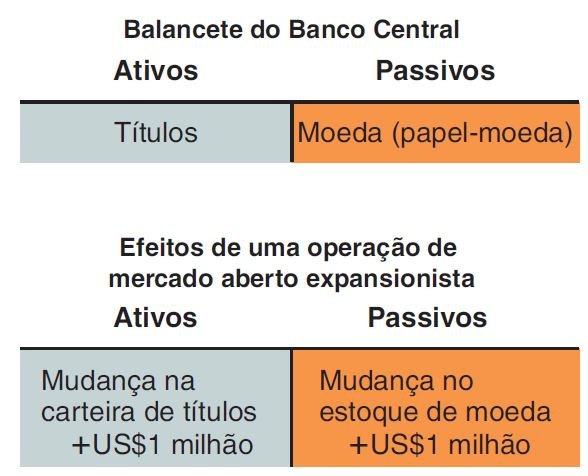
\includegraphics[width=0.55\textwidth]{./figures/aula072_fig5.JPG}
    \caption{Balancete patrimonial do Banco Central. Fonte: Blanchard (2017).}
    \label{fig5}
\end{figure}
\end{frame}

\begin{frame}{Preço $\times$ rendimento de títulos}
    \begin{itemize}
        \item Na realidade, o que é determinado nos mercados de títulos não são as taxas de juros, mas os \hlight{preços} dos títulos
        \bigskip
        \item No entanto, os preços de títulos e suas taxas de juros estão diretamente relacionados
        \bigskip
        \item Suponhamos que os títulos em nossa economia sejam de um ano - títulos que prometem pagar uma certa quantidade de moeda daqui um ano
        \bigskip
        \item Nos EUA, títulos emitidos pelo governo com promessa de pagamento em um ano ou menos são chamados de \textbf{letras do Tesouro} ou, simplesmente, \textbf{T-bills}
    \end{itemize}
\end{frame}

\begin{frame}{Preço $\times$ rendimento de títulos}
\begin{itemize}
    \item Suponha um título que promete pagar $\$ 100$ daqui a um ano. Seja o preço deste título hoje igual a $\$ P_B$. Se um indivíduo comprar este título hoje e o mantiver por um ano, a taxa de retorno da posse do título por um ano será igual a $(\$ 100 - \$P_B)/\$ P_B$. Portanto, a taxa de juros do título é dada por:
    \[
    i = \frac{\$ 100 - \$P_B}{\$P_B}.
    \]
    Ou seja, \textbf{quanto maior for o preço do título, menor será a taxa de juros}.
    \bigskip
    \item Se soubermos a taxa de juros, podemos descobrir o preço do título:
    \[
    \$P_B = \frac{\$100}{1 + i}.
    \]
    Se a taxa de juros é positiva, o preço do título é menor que o pagamento final. \textbf{Quanto maior a taxa de juros, menor o preço atual do título}.
\end{itemize}
\end{frame}

\begin{frame}{Operações de mercado aberto}
    \begin{itemize}
        \item Ao realizar uma operação de mercado aberta expansionista, o BC compra títulos no mercado de títulos e paga por eles por meio da criação de moeda
        \bigskip
        \item À medida que o BC compra títulos, a demanda por títulos cresce, aumentando seus preços
        \bigskip
        \item Reciprocamente, a taxa de juros dos títulos cai
        \bigskip
        \item Note que, ao comprar títulos em troca da moeda que criou, o BC expandiu a base monetária
        \bigskip
        \item Portanto, ao comprar ou vender títulos em troca de moeda, o BC afeta o preço dos títulos e, consequentemente, a taxa de juros sobre os títulos
    \end{itemize}
\end{frame}

\begin{frame}{Resumo}
    \begin{itemize}
        \item A taxa de juros é determinada pela igualdade entre oferta e demanda por moeda
        \bigskip
        \item Ao alterar a oferta de moeda, o BC pode afetar a taxa de juros
        \bigskip
        \item O BC altera a oferta de moeda por meio de operações de mercado aberto, que são compras ou vendas de títulos em troca de moeda
        \bigskip
        \item As operações de mercado aberto nas quais o BC aumenta a oferta de moeda por meio da compra de títulos levam a um aumento nos preços dos títulos e a uma diminuição na taxa de juros. A curva de oferta de moeda é deslocada para direita
        \bigskip
        \item As operações de mercado aberto nas quais o BC diminui a oferta de moeda por meio da venda de títulos levam a uma diminuição no preço dos títulos e a um aumento na taxa de juros. A curva de oferta de moeda é deslocada para esquerda
    \end{itemize}
\end{frame}

\section{Oferta de moeda $\times$ taxa de juros}
\subsection{Regras de taxa de juros $\times$ regras de estoque de moeda}
\begin{frame}{Regras de taxa de juros $\times$ regras de estoque de moeda}
\begin{itemize}
    \item Vimos que o BC escolhe a oferta de moeda e deixa a taxa de juros ser determinada no ponto em que a oferta de moeda iguala a demanda por moeda
    \bigskip
    \item Poderíamos, alternativamente, ter descrito que o BC escolhe a taxa de juros e, então, ajusta a oferta de moeda de modo a atingir essa taxa de juros
    \bigskip
    \item Vimos o efeito de uma decisão do BC de aumentar a oferta de moeda de $M^s$ para $M^{s'}$, causando uma queda da taxa de juros de $i$ para $i^{'}$
    \bigskip
    \item Poderíamos ter descrito em termos de uma decisão do BC de diminuir a taxa de juros de $i$ para $i^{'}$ por meio de um aumento da oferta de moeda de $M^s$ para $M^{s'}$
\end{itemize}
\end{frame}

\begin{frame}{Regras de taxa de juros $\times$ regras de estoque de moeda}
    \begin{figure}
        \centering
        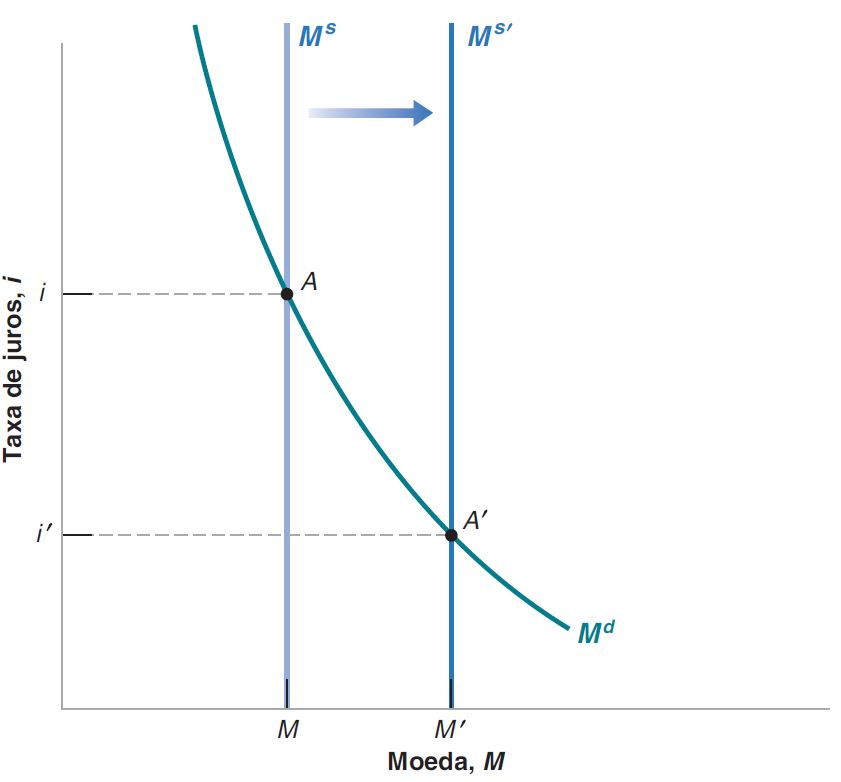
\includegraphics[width=0.5\textwidth]{./figures/aula072_fig4.JPG}
        \caption{Instrumento do Banco Central - estoque de moeda $\times$ taxa de juros. Fonte: Blanchard (2017).}
        \label{fig6}
    \end{figure}
\end{frame}

\begin{frame}{Regras de taxa de juros $\times$ regras de estoque de moeda}
    \begin{itemize}
        \item Por que é útil pensar na escolha da taxa de juros?
        \bigskip
        \item Porque é o que os BCs, incluindo o BACEN e o Fed, normalmente fazem
        \bigskip
        \item Eles normalmente pensam na taxa de juros que desejam atingir e, então, alteram a oferta de moeda de modo a atingir essa taxa
        \bigskip
        \item No noticiário não ouvimos: ``O BC decidiu restringir a oferta de moeda hoje.'' E, sim, que: ``O BC decidiu aumentar a taxa de juros hoje''
        \bigskip
        \item O BC faz isso por meio de uma redução adequada da oferta de moeda
        \hyperlink{apendice}{\beamerbutton{Apêndice}}
    \end{itemize}
\end{frame}

\section{Determinação da taxa de juros (II)}
\subsection{Introdução}
\begin{frame}{Introdução}\label{voltar}
    \begin{itemize}
        \item Até agora consideramos apenas a Base Monetária Restrita (M0): papel-moeda emitido e reservas bancárias
        \bigskip        
        \item Agora examinaremos como a introdução dos depósitos à vista (ofertados pelos bancos comerciais) muda nossas conclusões
        \bigskip
        \item Ponto fundamental: mesmo neste caso mais complicado, ao mudar o montante de moeda, o BC pode controlar a taxa de juros e, assim, o faz
        \bigskip
        \item Para entender o que determina a taxa de juros de uma economia quando consideramos o agregado monetário M1 (papel-moeda e depósitos à vista), precisamos examinar primeiro o que os bancos fazem
    \end{itemize}
\end{frame}

\subsection{O que os bancos fazem}
\begin{frame}{O que os bancos fazem}
    \begin{itemize}
        \item Economias modernas são caracterizadas pela existência de muitos tipos de \textcolor{blue}{intermediários financeiros} - instituições que recebem fundos de famílias e firmas e os usam para comprar ativos financeiros ou para fazer empréstimos a outras pessoas e firmas
        \bigskip
        \item O ativo dessas instituições é composto de ativos financeiros que possuem e de empréstimos que fizeram
        \bigskip
        \item O passivo é o que devem a pessoas e firmas de quem receberam fundos
        \bigskip
        \item Os \textbf{bancos} são um tipo de intermediário que, em especial, possuem passivos em forma de moeda: as pessoas podem pagar por transações emitindo cheques até o montante de seu saldo em conta
    \end{itemize}
\end{frame}

\begin{frame}{O que os bancos fazem}
    \begin{figure}
        \centering
        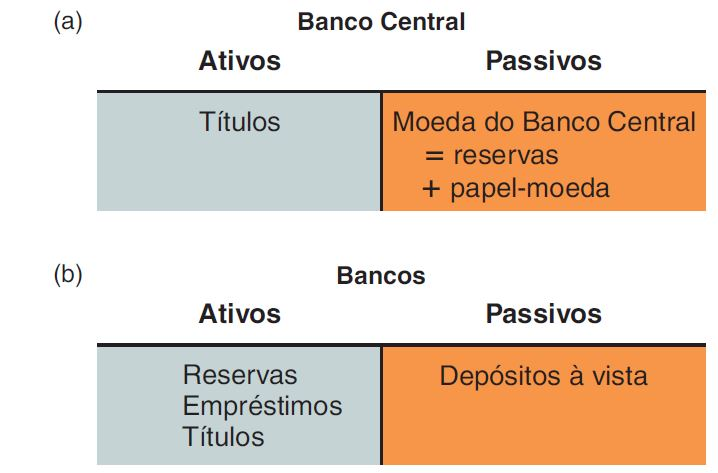
\includegraphics[width=0.7\textwidth]{./figures/aula072_fig6.JPG}
        \caption{Balanço patrimonial de bancos privados e BC. Fonte: Blanchard (2017).}
        \label{fig7}
    \end{figure}
\end{frame}

\begin{frame}{O que os bancos fazem}
    \begin{itemize}
        \item Bancos recebem fundos de pessoas e empresas, que ou os depositam diretamente ou solicitam que os fundos sejam enviados às suas contas-correntes. Pessoas e empresas podem emitir cheques ou fazer retiradas até o montante total de seus saldos em conta a qualquer momento. Consequentemente, \textcolor{red}{o passivo dos bancos é igual ao valor desses depósitos à vista}
        \bigskip
        \item Com relação ao BC, o ativo continua sendo o mesmo - soma dos títulos que ele retém
        \bigskip
        \item No entanto, no lado do passivo, nem toda moeda do BC emitida é mantida como papel-moeda pelo público. Agora, parte dela é mantida como reservas pelos bancos comerciais
    \end{itemize}
\end{frame}

\begin{frame}{O que os bancos fazem}
    \begin{itemize}
        \item Os bancos mantêm como \textbf{reservas} parte dos fundos que recebem. Essas reservas são mantidas parcialmente em dinheiro e parcialmente em uma conta mantida no BC, da qual podem fazer retiradas quando necessário. Por que manter reservas?\bigskip
        \begin{enumerate}
            \item O montante de saques diários não é necessariamente igual ao montante de depósitos diários. Portanto, o banco deve sempre manter algum dinheiro à disposição
            \medskip
            \item Diariamente, as pessoas com contas no banco emitem cheques para pessoas com contas em outros bancos, e pessoas com contas em outros bancos emitem cheques para pessoas com contas no banco. Como resultado dessas transações, o montante que um banco deve a outros bancos pode ser maior ou menor que o montante que outros bancos o devem. Portanto, o banco deve manter reservas
            \medskip
            \item Os bancos são sujeitos a recolhimentos \textbf{compulsórios} que os obrigam a manter reservas em alguma proporção de seus depósitos à vista
        \end{enumerate}
    \end{itemize}
\end{frame}

\begin{frame}{O que os bancos fazem}
    \begin{itemize}
        \item EUA: recolhimentos compulsórios eram determinados pelo Fed e a alíquota era de 10\% do valor dos depósitos à vista
        \bigskip
        \item Os 90\% restantes poderiam ser usados para fazer empréstimos ou comprar títulos
        \bigskip
        \item Os empréstimos representam cerca de 70\% do ativo dos bancos, excluindo-se as reservas
        \bigskip
        \item Os títulos correspondem a 30\%
        \bigskip
        \item A distinção entre títulos e empréstimos é importante para questões como ``corridas bancárias'' e o papel do seguro de depósito federal (EUA)/Fundo Garantidor de Créditos (Brasil). Mas para o nosso objetivo, determinação da oferta de moeda, não é relevante
        \bigskip
        \item Portanto, vamos supor que os bancos não fazem empréstimos e que retêm como ativo apenas reservas e títulos
    \end{itemize}
\end{frame}

\subsection{Oferta e demanda por moeda do Banco Central}
\begin{frame}{Oferta e demanda por moeda do BC}
    \begin{itemize}
        \item Como considerar o equilíbrio nesse cenário mais realista?
        \bigskip
        \item Em termos da oferta e demanda por moeda do BC
        \bigskip
        \item A demanda por moeda do BC é igual à demanda por papel-moeda pelas pessoas mais a demanda por reservas pelos bancos
        \bigskip
        \item A oferta de moeda continua sob controle direto do BC
        \bigskip
        \item A taxa de juros de equilíbrio é a que equaliza demanda e oferta de moeda do BC
    \end{itemize}
\end{frame}

\begin{frame}{Demanda por moeda do BC}
    \begin{itemize}
        \item Demanda por moeda do BC: demanda por moeda por parte das pessoas e demanda por reservas por parte dos bancos
        \bigskip
        \item Para simplificar, vamos assumir que as pessoas preferem ter moeda em forma de depósitos à vista e não possuem papel-moeda
        \bigskip
        \item O caso mais geral é tratado no apêndice do capítulo 4 de Blanchard (2017) e leva às mesmas conclusões básicas
        \bigskip
        \item Portanto,  a demanda por moeda do BC é igual à demanda por reservas pelos bancos
        \bigskip
        \item Esta demanda, por sua vez, depende da demanda por depósitos à vista por parte das pessoas
        \bigskip
        \item Temos, então, que a demanda por depósitos à vista é igual à demanda por moeda por parte das pessoas (já que elas não detêm papel-moeda)
    \end{itemize}
\end{frame}

\begin{frame}{Demanda por moeda do BC}
    \begin{itemize}
        \item A demanda por depósitos à vista é, então, descrita pela mesma equação que vimos anteriormente:
        \begin{equation}
            M^d = \$Y L(i), \qquad L'(i)<0.
        \end{equation}
        As pessoas querem manter mais depósitos à vista quanto maior for o nível de transações e menor a taxa de juros sobre os títulos
        \bigskip
        \item Quando consideramos a demanda por reservas por parte dos bancos, quanto maior o montante de depósitos à vista, maior o montante de reservas que os bancos devem deter, tanto por precaução quanto para fins regulatórios
        \bigskip
        \item Seja $\theta$ a \textbf{razão das reservas}, o montante de reservas que os bancos possuem por unidade monetária de depósitos à vista
        \bigskip
        \item Então, a demanda por reservas por parte dos bancos comerciais é dada por:
        \begin{equation}
            H^d = \theta M^d = \theta \$Y L(i).
            \label{eq4}
        \end{equation}
    \end{itemize}
\end{frame}

\begin{frame}{Demanda por moeda do BC}
    \begin{equation*}
        H^d = \theta M^d = \theta \$Y L(i).        
    \end{equation*}
    \bigskip
    \begin{itemize}
        \item Letra $H$: moeda do BC é às vezes chamada de \textcolor{blue}{base monetária} (\emph{high-powered money}) para refletir seu papel na determinação da taxa de juros de equilíbrio
        \bigskip
        \item Primeira igualdade: a demanda por reservas é proporcional à demanda por depósitos à vista
        \bigskip
        \item Segunda igualdade: a demanda por depósitos à vista depende da renda nominal e da taxa de juros
        \bigskip
        \item Logo, a demanda por moeda do BC, equivalente à demanda por reservas dos bancos, é igual à $\theta$ vezes a demanda por moeda por parte das pessoas
    \end{itemize}
\end{frame}

\begin{frame}{Equilíbrio no mercado de moeda do BC}
    \begin{itemize}
        \item A condição de equilíbrio é que a oferta de moeda do BC seja igual à sua demanda por moeda
        \bigskip
        \item A oferta de moeda do BC ($H$) - equivalente à oferta de reservas pelo BC - está sob controle direto da autoridade monetária e pode ser alterada por meio de operações de mercado aberto
        \bigskip
        \item Portanto:
        \[
            H = H^d,
        \]
        ou, ainda:
        \begin{equation}
            H = \theta \$Y L(i).
            \label{eq7}
        \end{equation}
    \end{itemize}
\end{frame}

\begin{frame}{Equilíbrio no mercado de moeda do BC}
    \begin{figure}
        \centering
        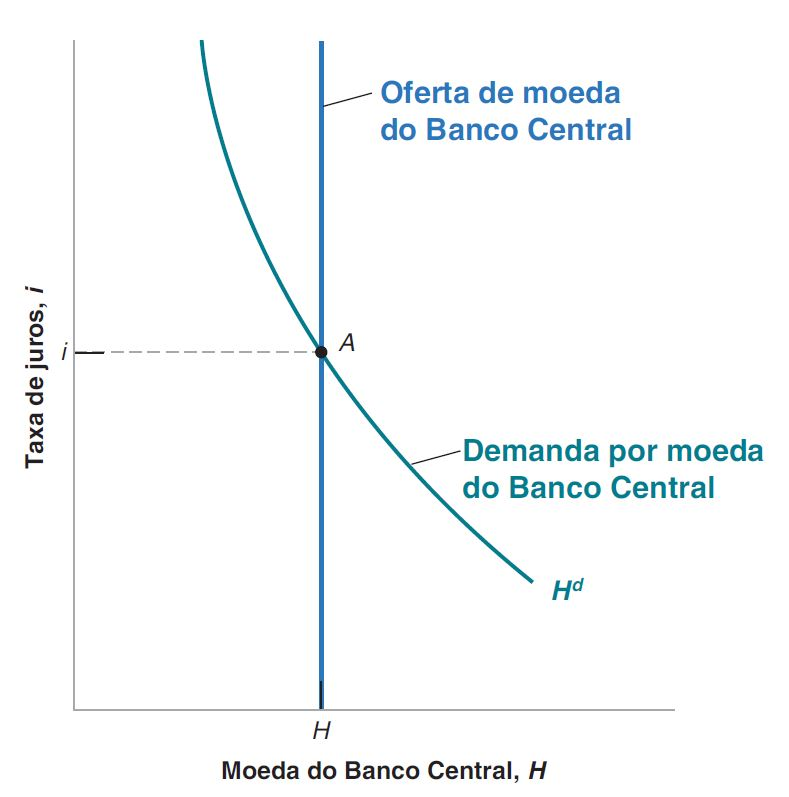
\includegraphics[width=0.45\textwidth]{./figures/aula072_fig7.JPG}
        \caption{Equilíbrio no mercado de moeda do BC e determinação da taxa de juros. Fonte: Blanchard (2017).}
        \label{fig8}
    \end{figure}
\end{frame}

\begin{frame}{Equilíbrio no mercado de moeda do BC}
    \begin{itemize}
        \item A condição de equilíbrio da equação (\ref{eq7}) é representada graficamente pela Figura \ref{fig8}. No eixo horizontal temos a moeda do BC e, no vertical, a taxa de juros
        \bigskip
        \item A demanda por moeda do BC, $H^d$, é traçada para um dado nível de renda nominal $\$ Y$
        \bigskip
        \item Uma taxa de juros mais alta implica uma demanda mais baixa por moeda do BC à medida que diminuem a demanda por depósitos à vista por parte das pessoas e, assim, a demanda por reservas por bancos
        \bigskip
        \item Os efeitos das variações da renda nominal e da oferta de moeda do BC são qualitativamente os mesmos que vimos anteriormente
        \bigskip
        \item Assim, a conclusão básica é a mesma: \textbf{ao controlar a oferta de moeda do BC, este pode determinar a taxa de juros sobre títulos}
    \end{itemize}
\end{frame}

\section{Resumo}
\begin{frame}{Resumo}
\begin{itemize}
    \item A demanda por moeda depende positivamente do nível de transações na economia e negativamente da taxa de juros: $M^d = \$YL(i)$
    \bigskip
    \item A taxa de juros é determinada pela condição de equilíbrio de que a oferta seja igual à demanda por moeda: $M = M^d$
    \bigskip
    \item Para $M^s$ fixo, um aumento da renda leva a um aumento da demanda por moeda e a um aumento da taxa de juros. Um aumento da oferta de moeda, para dada renda, leva a uma diminuição da taxa de juros
    \bigskip
    \item A forma como o BC altera a oferta de moeda consiste nas operações de mercado aberto
    \bigskip
    \item Operações expansionistas (contracionistas) de mercado aberto levam a um aumento (diminuição) do preço dos títulos e a uma diminuição (aumento) da taxa de juros
\end{itemize}    
\end{frame}

\begin{frame}{Resumo}
    \begin{itemize}
        \item Quando a moeda inclui tanto papel-moeda quanto depósitos à vista, podemos pensar na taxa de juros como determinada pela condição de que a oferta de moeda do BC seja igual à demanda por sua moeda
        \bigskip
        \item A oferta de moeda do BC está sob o controle da autoridade monetária. No caso especial em que as pessoas retêm apenas depósitos à vista, a demanda por moeda do BC é igual à demanda por reservas pelos bancos comerciais, que é, por sua vez, igual à demanda total por moeda multiplicada pela razão das reservas escolhida pelos bancos
    \end{itemize}
\end{frame}

\section{Apêndice}
\begin{frame}{Taxa de juros $\times$ oferta de moeda}\label{apendice}
    \begin{itemize}
        \item Muitas das tradicionais prescrições de política monetária focam no estoque de moeda
        \bigskip
        \item Por exemplo, Friedman (1960) e outros argumentam que o BC deveria seguir uma \textcolor{blue}{regra do $k$-porcento}
        \bigskip
        \item Isto é, os formuladores de política econômica deveriam ter como objetivo manter o estoque de moeda crescendo de maneira constante a uma taxa anual de $k$ porcento (onde $k$ é um número pequeno, e.g., 2 ou 3). E, assim, renunciar a tentativas de estabilizar a economia
        \bigskip
        \item Estas regras de controle da oferta monetária possuem um apelo considerável
        \bigskip
        \item O crescimento da moeda, como vimos no modelo clássico e veremos mais adiante, é um determinante fundamental da inflação no longo prazo
        \bigskip
        \item Além disso, é via ajustes do estoque de moeda que o BC altera a taxa de juros
    \end{itemize}
\end{frame}

\begin{frame}{Taxa de juros $\times$ oferta de moeda}
    \begin{itemize}
        \item No entanto, apesar da defesa de regras de estoque de moeda por parte de muitos economistas, os BCs dão um foco muito pequeno ao estoque de moeda na condução de políticas monetárias
        \bigskip
        \item As medidas de estoque de moeda que o Banco Central tem amplo controle não estão intimamente ligadas à demanda agregada
        \bigskip
        \item E as medidas de estoque de moeda que estão mais intimamente ligadas à demanda agregada, como $M2$, são de difícil controle por parte do BC. Ver \href{https://pt.wikipedia.org/wiki/Base_monet\%C3\%A1ria}{composição da base monetária}
        \bigskip
        \item Além disso, em muitos países, a relação entre as medidas de estoque de moeda e demanda agregada foram rompidas nas décadas recentes, enfraquecendo a defesa por regras de estoque de moeda ainda mais
    \end{itemize}
\end{frame}

\begin{frame}{Taxa de juros $\times$ oferta de moeda}
    \begin{itemize}
        \item Devido a essas dificuldades, os BCs modernos raramente conduzem política monetária tentando atingir uma meta de taxa de crescimento para o estoque de moeda
        \bigskip
        \item Ao invés disso, suas políticas são focadas em ajustes da taxa nominal de juros de curto prazo (e.g., SELIC) em resposta a vários distúrbios na economia
        \bigskip
        \item Nos bastidores, no entanto, o que permite que eles façam isso é o controle que detem sobre a oferta de moeda
    \end{itemize}
\end{frame}

\begin{frame}{Taxa de juros $\times$ oferta de moeda}
    \begin{itemize}
        \item Taylor (1993) e Bryant, Hooper e Mann (1993) argumentam que a condução da política monetária deve ser pensada em termos de \textcolor{blue}{regras para a taxa nominal de juros de curto prazo}
        \bigskip
        \item Isto é, nunca devemos pensar em um BC que escolhe uma trajetória para a taxa de juros nominal que não seja responsiva às condições econômicas (isso levaria a instabilidade ou indeterminância), nem em ajustes da taxa de juros de maneira \emph{ad hoc}
        \bigskip
        \item Ao invés disso, devemos pensar no BC seguindo uma política de ajustes da taxa de juros de forma previsível a variações dos desenvolvimentos das condições econômicas
        \bigskip
        \item Mesmo que nenhuma das regras capture totalmente o comportamento dos BCs, essas regras de taxas de juros podem fornecer uma aproximação razoável para o comportamento dos BCs e podem ser analisadas formalmente
    \end{itemize}
\end{frame}

\begin{frame}{Regra de Taylor}
    \begin{itemize}
        \item Provavelmente, a regra mais famosa de taxa de juros é a proposta por Taylor
        \bigskip
        \item A \textcolor{blue}{regra de Taylor} é composta por dois componentes:
        \bigskip
        \begin{enumerate}
            \item A taxa nominal de juros deve crescer em uma proporção maior que um pra um com relação à inflação, ou seja, a taxa de juros real cresce quando a inflação aumenta
            \medskip
            \item A taxa nominal de juros deve crescer quando o produto agregado está acima do seu nível normal, e decrescer quando o produto estiver abaixo
        \end{enumerate}
        \bigskip
        \item Formalmente, a regra de Taylor pode ser enunciada da seguinte forma:
        \begin{equation}
            i_t = r^n + \phi_\pi (\pi_t -\pi^*) + \phi_y\left(\ln Y_t - \ln Y_t^n\right), \qquad \phi_\pi>1, \phi_y>0.
            \label{ap1}
        \end{equation}
    \end{itemize}
\end{frame}

\begin{frame}{Regra de Taylor}
    \begin{itemize}
        \item Taylor argumenta que uma regra como a definida em (\ref{ap1}) com $\phi_\pi = 1.5$, $\phi_y = 0.5$ e $r^n = \pi^* = 2\%$ fornece uma boa descrição para a política monetária norte-americana para o período 1985-2008
        
        \hyperlink{voltar}{\beamerbutton{Voltar}}
    \end{itemize}
    \end{frame}

\section{Bibliografia}
\begin{frame}{\emoji{books} Bibliografia}
    \begin{itemize}
        \item BLANCHARD, O. Macroeconomia. 7.ed. São Paulo: Pearson Education do Brasil, 2017\medskip        
        \item CARLIN, W.; SOSKICE, D. Macroeconomics: Institutions, instability, and the financial system. Oxford, UK: Oxford University Press, 2015\medskip
        \item DORNBUSCH, R.; FISCHER, S.; STARTZ, R. Macroeconomia. 11.ed. Porto Alegre: AMGH, 2013. Disponível em: \href{https://app.minhabiblioteca.com.br/books/9788580551853}{app.minhabiblioteca.com.br/books/9788580551853}\medskip
        \item MISHKIN, F.S. The economics of money, banking, and financial markets. 11.ed. Pearson Education Limited, England, 2016.
    \end{itemize}
\end{frame}
\end{document}